% Chapter Template

\chapter{Experimental Setup} % Main chapter title

\label{Chapter3} % Change X to a consecutive number; for referencing this chapter elsewhere, use \ref{ChapterX}
In the following chapter, we will look in detail the components of the experimental 
setup to observe the effects of different spatial correlations in a lensless quantum image
experiment. The setup consist of two  main stages. The first one is the light source 
with tunable spatial correlations, and the second one the two-photon imaging system. 
This experimental setup located at the optical table of the 
Quantum Optics Laboratory.
%----------------------------------------------------------------------------------------
%	SECTION 1
%----------------------------------------------------------------------------------------
\section{Light Source with Tunable Spatial Correlations}

The experimental setup to obtain pairs of photons is shown in Figure \ref{fig:SPDC}. 
The source consists of a type-II crystal in  non-collinear configuration. The source is based
on spontaneous parametric down conversion.


\begin{figure}[h!]
\centering
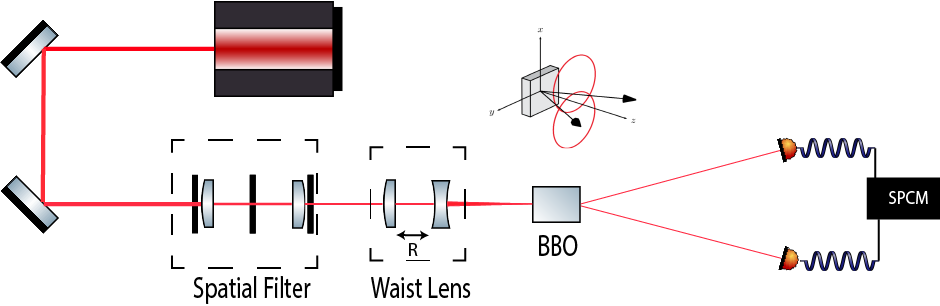
\includegraphics[width=0.8\textwidth]{Figures/SPDC.png}
\caption{Experimental Setup for the SPDC light Source} 
\label{fig:SPDC}
\end{figure}


To obtain pairs of photons by means of SPDC, we need to pump a nonlinear crystal.
For this experiment, we use a diode laser (Crystal Laser model No. DL 405-200),  
that delivers a continuous wave(CW) at wavelength $\lambda = 406,101 nm$ and $\Delta \lambda = 4 nm$. 
The laser delivers light at 200 mW with a beam diameter 
of 1.5 mm and a beam Divergence of 1.2 mrad.






As seen in Figure \ref{fig:SPDC}, we redirect the laser beam two times, for doing
so we use a pair of mirrors. For this kind of experiments, when the efficiency 
of the optical elements is really important, it is important to use the correct type
of mirror, we want a mirror that reflects most of the light. For this reason, depending
on the wavelength it is posible to find mirrors and lenses with different types of 
coating. Mirror and Lenses have a thin layer that is more efective for a range 
of wave lengths. For our experiment the mirrors have a coating that highly reflects light at
$405nm$. It is posible to manipulate the direction in which the mirror will reflect the 
light by using an appropriate mount with screws that allows to move the reflected beam in one
direction. In the experimental setup we use two mirrors to change the direction two times.



\subsection{Spatial Filter to achieve a Gaussian pump beam}
As seen in theory we need a gaussian beam to pump the crystal. In our experiment we have a 
diode laser whose spatial profile is not a Gaussian. This ramdom spatial profile is a result of the randomnes in the quantum emissions and 
absorptions that are happening at the exited atoms at the diode laser\cite{hecht}.
In order to achieve a Gaussian profile, we use the spatial filter presented in the 
Figure \ref{fig:SPDC}. The spatial filter is composed by two irises, an Aspheric Lens of $f=30 mm$(LA1805-A), a pinhole of $50 \mu m$ and a 
collimating lens of $f=60 mm$(LA1134-A).
\begin{figure}[h!]
\centering
{  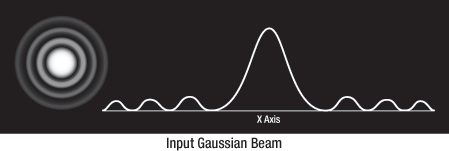
\includegraphics[width=0.6\textwidth]{Figures/inputBeam.png} }
{  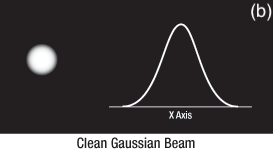
\includegraphics[width=0.6\textwidth]{Figures/outputBeam.png} }
\caption{The spatial intensity profile before and after the spatial filtering process , Taken from \cite{thorlabs}}
 \label{fig:inputOutputBeam}
\end{figure}

To undestand what a spatial filter does consider a light beam with a spatial profile as the 
one depicted in Figure \ref{fig:inputOutputBeam}(a). After passing a spatial filter the 
obtained light beam look like the one in Figure \ref{fig:inputOutputBeam}(b), that is 
now the Gaussian profile we were looking for.

In Figure \ref{fig:int} we can appreciate the spatial intensity profile of the pump beam just after 
it goes through the spatial filter, the red line is a fit done computationally. The green dots are the measured waist at 3 given
percentages of intensity, $13.5\%$, $50\%$ and $80\%$ respectably. The tool we used to measure this is called Beam Master, and it have its own spatial directions, V and W direction . 
In the optical table we made sure that the V and W direction agreed with our x and y directions. The waist of a gaussian beam propagating in the z direction is given by\cite{waist}:
\begin{equation}\label{eq:wa}
w(z)=w_0 \sqrt{1+(z/z_R)^2}.
\end{equation}
Where $z_R$ is the \textit{Rayleigh length} and it's defined as $z_R=\frac{\pi n w_0^2}{\lambda_0}$. The previous expresion is a function 
of $n$ the refractive index, $\lambda_0$ the wavelength of the beam and $w_0=w(0)$ the waist at the origin. 
 


\begin{figure}[h!]
\centering
{  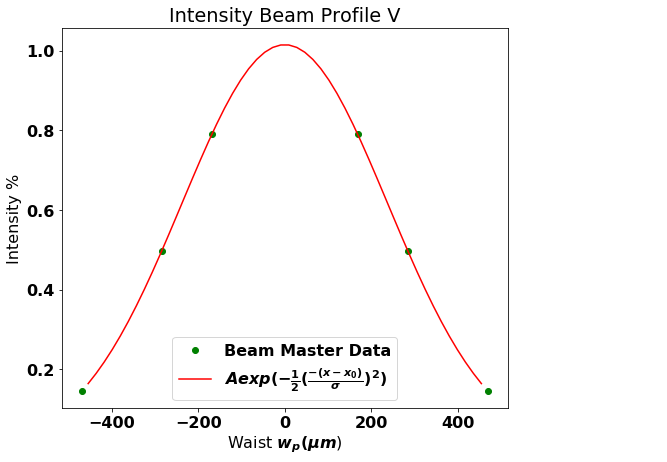
\includegraphics[width=0.48\textwidth]{Figures/inteV.png} }
{  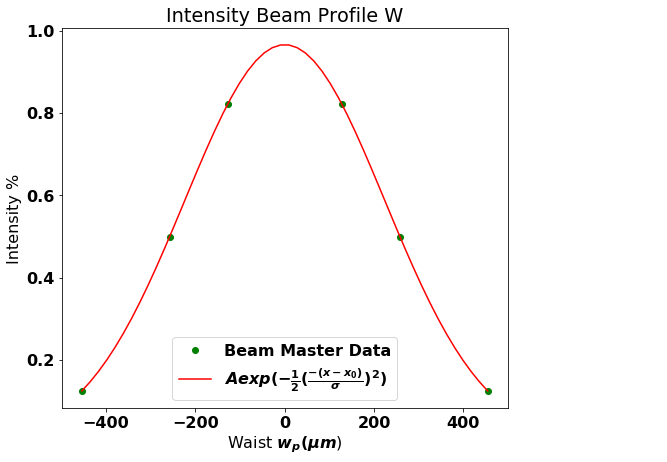
\includegraphics[width=0.48\textwidth]{Figures/inteW.png} }
\caption{The spatial intensity profile measured after the spatial filter}
 \label{fig:int}
\end{figure}



\subsection{Lenses to Control the pump beam waist}

After successfully achieving a Gaussian profile, which is important for the reasons 
described in Section \ref{sec:spatialCorrelations}, we need a way to control the pump waist, 
but we need to do it 
in a way not too complicated, that doesn't imply too many changes in the experimental setup.
 Putting a  lens, in the beam propagation direction, with certain focal lenght $f$ will define
 a zone around the distance $f$ called \textit{Focus depth}\cite{hecht}, where in the middle 
we find the narrowest point of the beam. The radius of this zone is:
\begin{equation}
 W_0=\frac{\lambda f}{\pi W_B}.
\end{equation}
Where $W_B$ is the width of beam at the lens. In Figure \ref{fig:waist} we see this 
behaviour.  If we want to change $W_0$, we need to use a different lens with $f'$ a different
focal length. This will produce also a different \textit{Focus depth}. Therefore, 
if we want to focus the beam at a fixed distance $F$, using this method to control the pump
 waist is not practical. Every different lens we would use will make this waist $W_0$ at a
 differents distances $f$. It is necessary to find a combination of lenses, that we will call
\textit{waist lens} that make us a 
$W_0$ at a transverse plane located in a fixed position $F$ from the set. 
In Figure \ref{fig:fixed} we present the combination of lenses, \textit{waist lens}.
 It consists on an arrangment of two 
lenses, a positive and a negative one, separated a distance $d_0$ from each other.
\begin{figure}[h!]
\centering
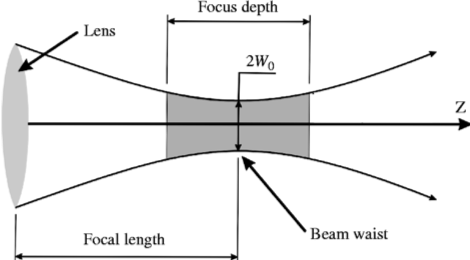
\includegraphics[width=0.5\textwidth]{Figures/waist.png}
\caption{Effect of lens on a Gaussian beam\cite{hecht}} 
\label{fig:waist}
\end{figure}


\begin{figure}[h!]
\centering
 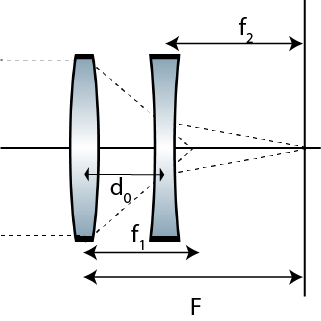
\includegraphics[width=0.65\textwidth]{Figures/fixed.png}
\caption{Composition of lenses to control the Pump Waist at a Fixed distance $F$} 
\label{fig:fixed}
\end{figure}
We can define a \textit{effective focal length} $F$ as a function of  $f_1$ and $f_2$, the focal lengths of the positive and negative lenses 
respectively. With the constrain that $d_0 < f_1$, $F$ reads:
\begin{equation}
F=\frac{f_1 |f_2|}{|f_2|-f_1+d_0}.
\end{equation}
This new effective focal length is crucial in the realisation of this experiment, as described before, we are interested in observing the effect 
in the reconstructed image using different spatial correlations. This is done by changing the pump waist of the laser that is focused on the crystal.
It is not experimentally practical to be changing the crystal position, it would mean to change the position of all the optical elements that 
follows. For this reason, it is perfect to be able to achieve the desired pump waist just by changing the relative separation of two lenses. 


\subsection{BBO(Beta Barium Borate) Crystal: The source of pair of photons}
The Beta Barium Borate (BBO) is an inorganic compound, with chemical formula $\beta$-BaB$_{2}$O$_4$. This crystal is a
nonlinear optical media commonly used. It is also a birefringent\footnote{Birefringence is a optical property of some materials of 
having a refractive index that depends on the polarisation and the propagation of light\cite{hecht}} material and its transmission regions extends
from $189nm$ to $3500nm$\cite{bbo}.
The type-II crystal is mounted is such way that the input and output plane are fixed. In particular the input plane is at $F$ from 
the \textit{waist lens} presented in the previous section, the power of the pump at this point is $\sim 60mW$. The generated photons doubles the wavelength 
of the original pump, it means the generated photon are around $810nm$.


\begin{comment}
\begin{figure}[h!]
\centering
{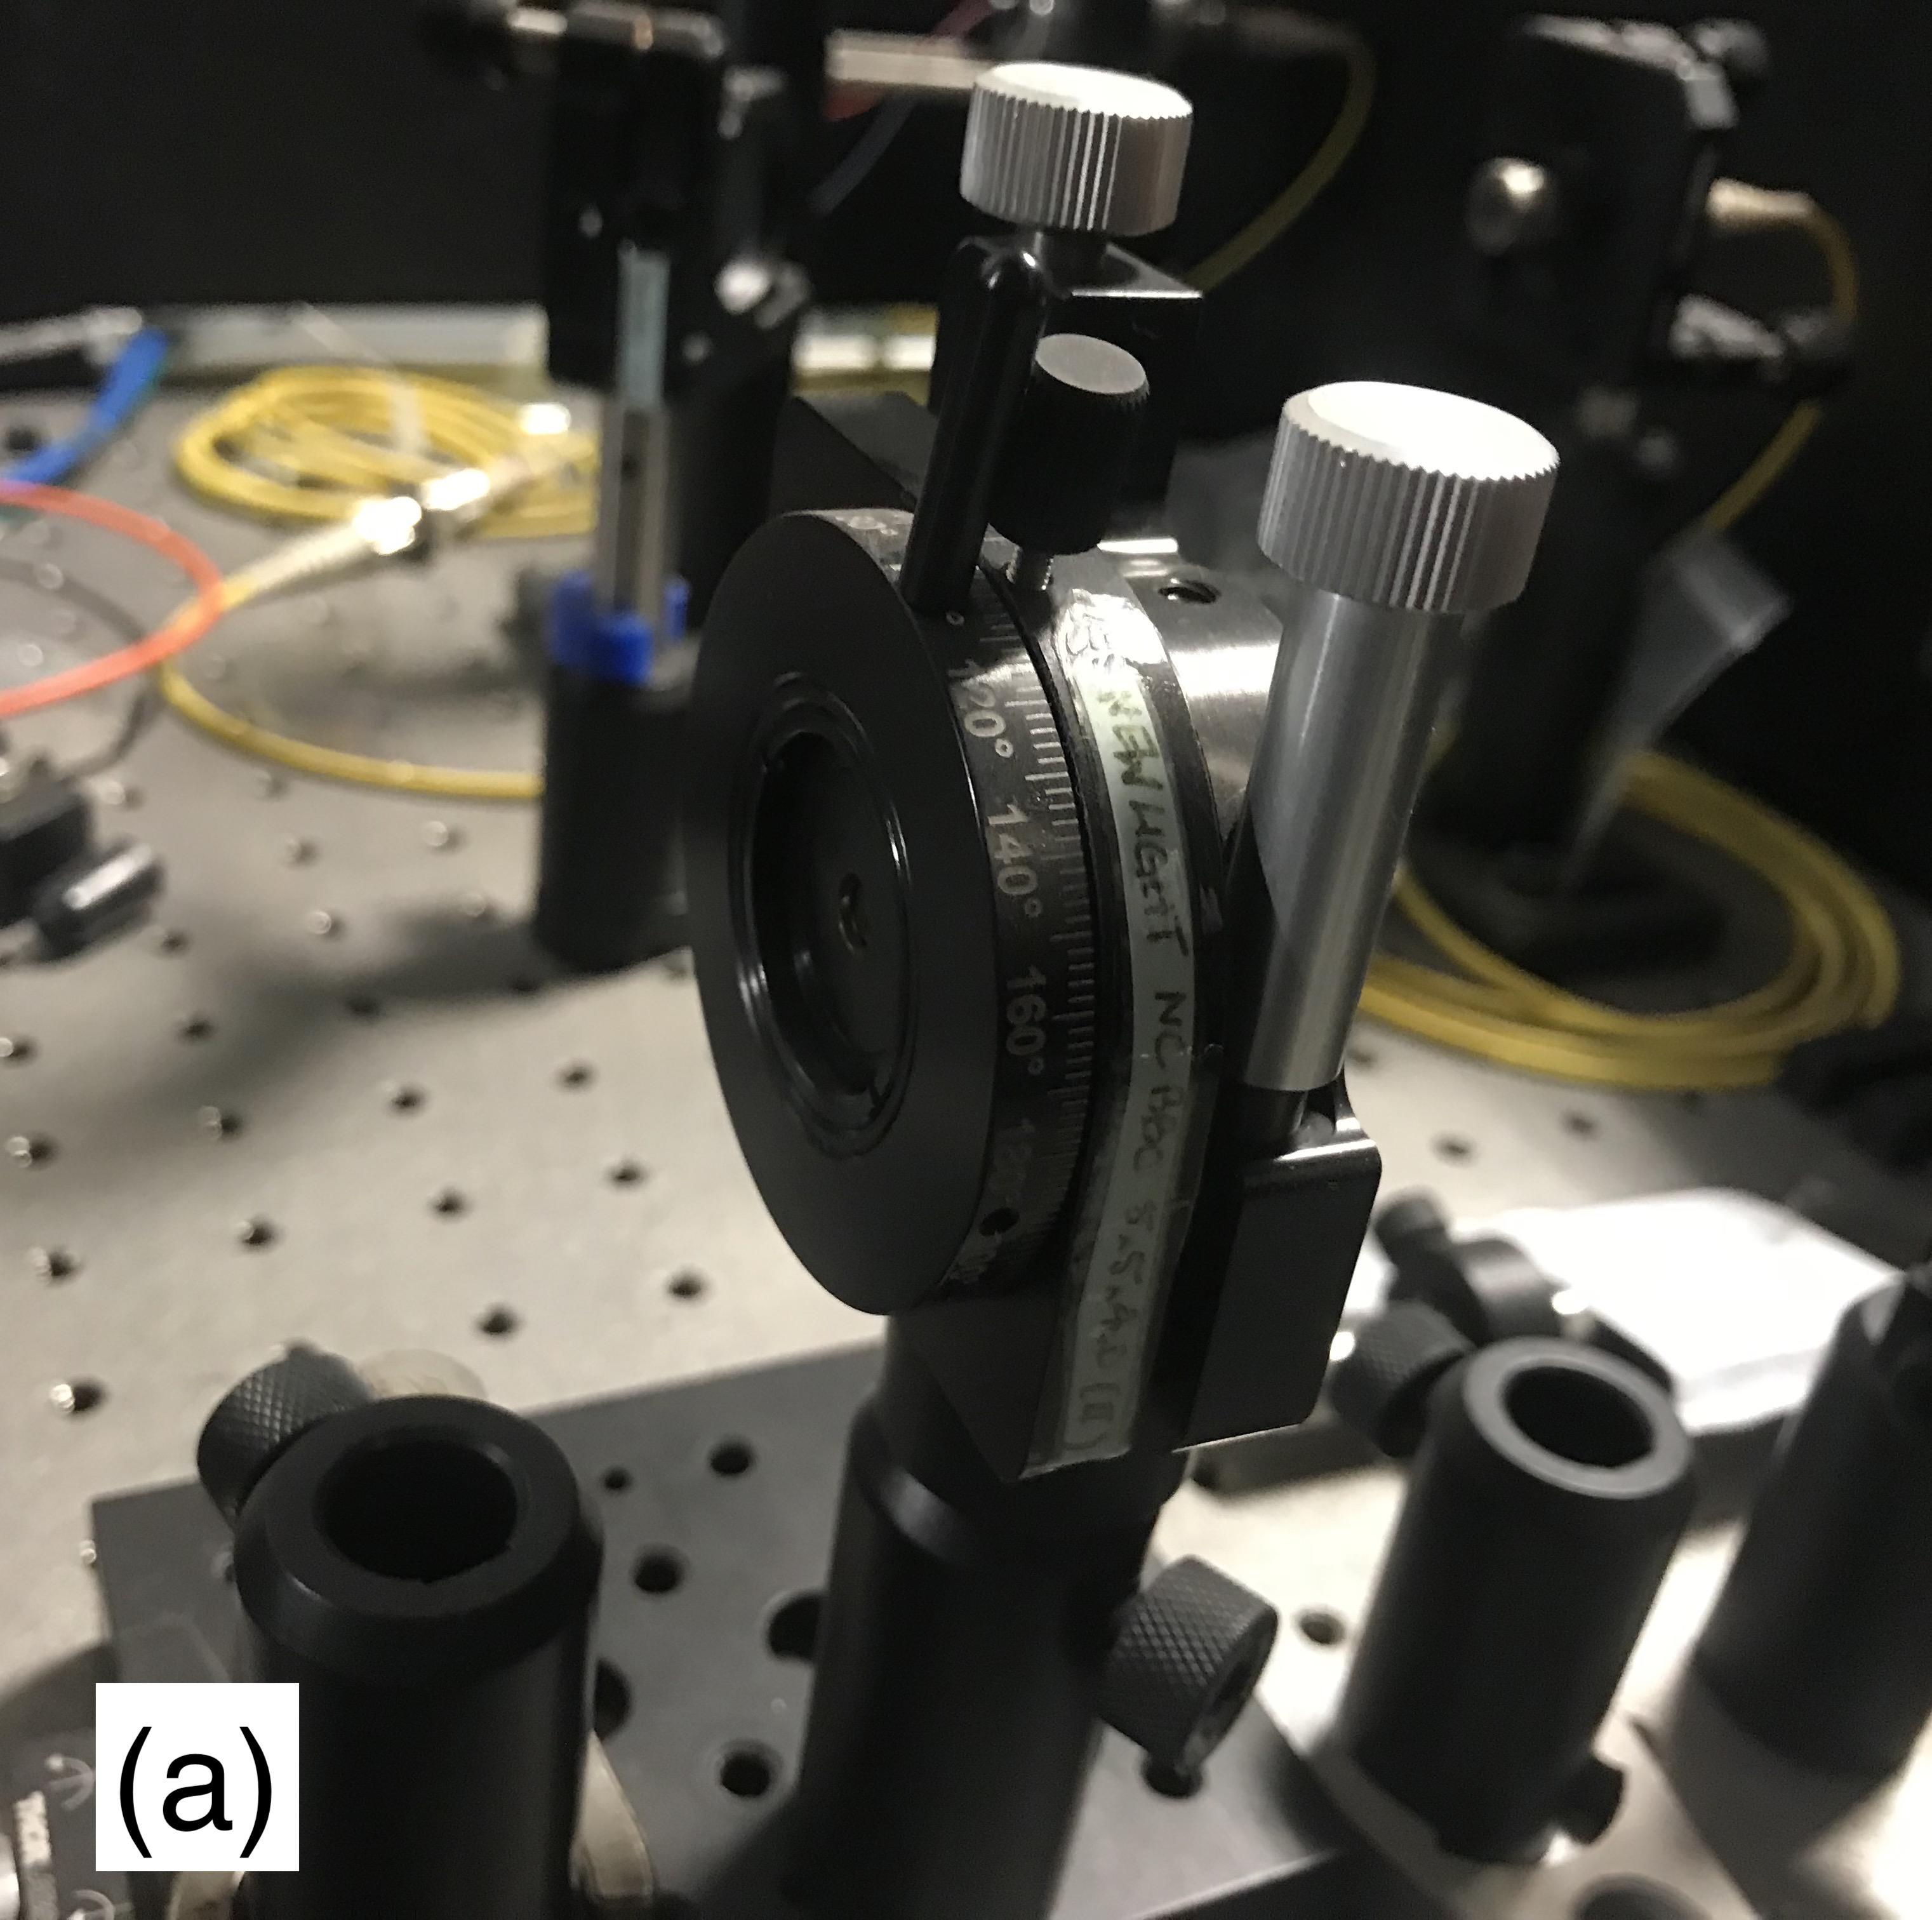
\includegraphics[width=0.35\textwidth]{Figures/bbo.jpg}}
{  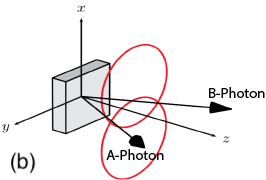
\includegraphics[width=0.5\textwidth]{Figures/aPhotonBPhoton.png} }
\caption{(a):Actual BBO crystal used in experiment. (b): the noncolinear configuration presented in this experiment}
 \label{fig:bbo}
\end{figure} 
\end{comment}

At this point we have as a result of the SPDC process a pair of entangled photons, which have an strong correlation. This correlation is 
the feature in which we are interested on. We need to observe the shape of this correlations functions and the next section will focus 
on the experimental setup that will allow us to observe this.



\section{Spatial Correlations Measurement Setup}\label{sec:pola}
From this point we will talk about a pair of correlated photons, that will come from the output plane of the BBO 
crystal, for historical reasons this photons are labeled as \textit{signal} and \textit{idler}. Nevertheless, to keep the same notations used through 
this monograph, this photon are going to be labeled as A-photon and B-photon, depending on which path they follow, in Figure \ref{fig:spatialSetup}
we can see the experimental setup for measuring the spatial correlations.

\begin{figure}[h!]
\centering
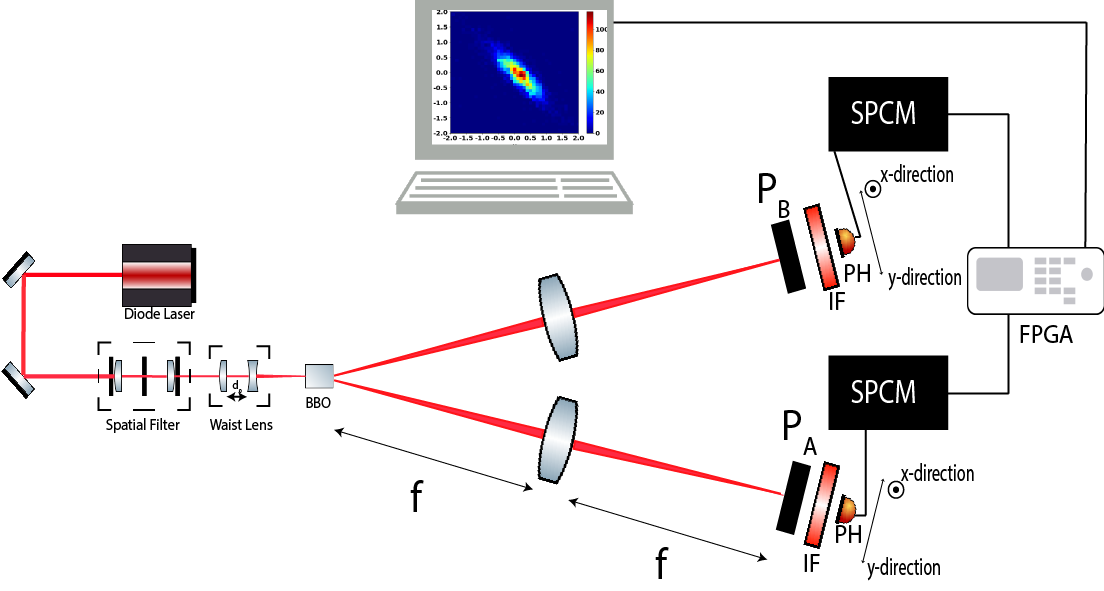
\includegraphics[width=1\textwidth]{Figures/spatialCorrelationSetup.png}
\caption{Experimental Setup for Obtaining the spatial correlations of a pair of down-converted photons} 
\label{fig:spatialSetup}
\end{figure}

Observing the theory developed before there is a relation between the transverse momentum $\vec{q}_n$ of the light before the 2-f system, and the photon 
position $\vec{r}_n$ after de system, Eq. \ref{eq:fourier}. For this reason we placed two lenses, one in each path of the light.
Doing this will put our detections in the Fourier plane. We use two lenses(LA1708) of $f=200.0mm$ in front 
of each \textit{A} and \textit{B}. It is also important to note that from now on, the lenses and mirror used from here, will have a coating that
transmits light around $810nm$ with high efficiency for the lenses, and highly reflects light at this wavelength. 




We are interested in just a pair photons, $\Phi(\vec{q}_B,\Omega_B;\vec{q}_A,\Omega_A)$, that are polarised in certain direction. In order to filter the others
photons $\Phi(\vec{q}_A,\Omega_A;\vec{q}_B,\Omega_B)$, and obtain the Eq. \ref{eq:stateFun}, we place a pair of polarisers at both paths. A polariser is an optical element that filters light
depending on the direction of the electrical field. We used a pair of Polarisers(WP25M-UB), which consist of an array of parallel metallic
wires sandwiched between glass with certain coating for better transmission.





As pointed out in Section \ref{sec:spatialCorrelations}, in order to observe the transverse
correlations, the frequency information has to be traced out. For doing so, we placed a 
pair of Interferometer Filters(IF), Thorlabs FB810-10. They are modeled as $f_n (\Omega_n)=\text{exp}[-\Omega_n^2/(
4\sigma_n^2)]$, where for this specific case $\Omega_n=810nm$ and $\sigma_n=2nm$. This optical elements 
have the special feature that only transmits light that comes throught this range of frequencies. 

\subsection{Detection Module}
To observe the spatial correlations we have to be able to measure light that is propagating
in the z-direction. Figure \ref{fig:scan} shows the plane that is being scanned, where each 
square have a $x_i$ and $y_j$ position, ${i,j}$ goes from $0$ to $N$. With the help of a motorised translational stages, we can make this $NxN$ steps. We can 
control the movement of a pin hole detector, which consists in a single mode optical fiber tip. The translational stages are controlled 
by Arduinos, this enable us to do the scan in a complete automated way.
\begin{figure}[h!]
\centering
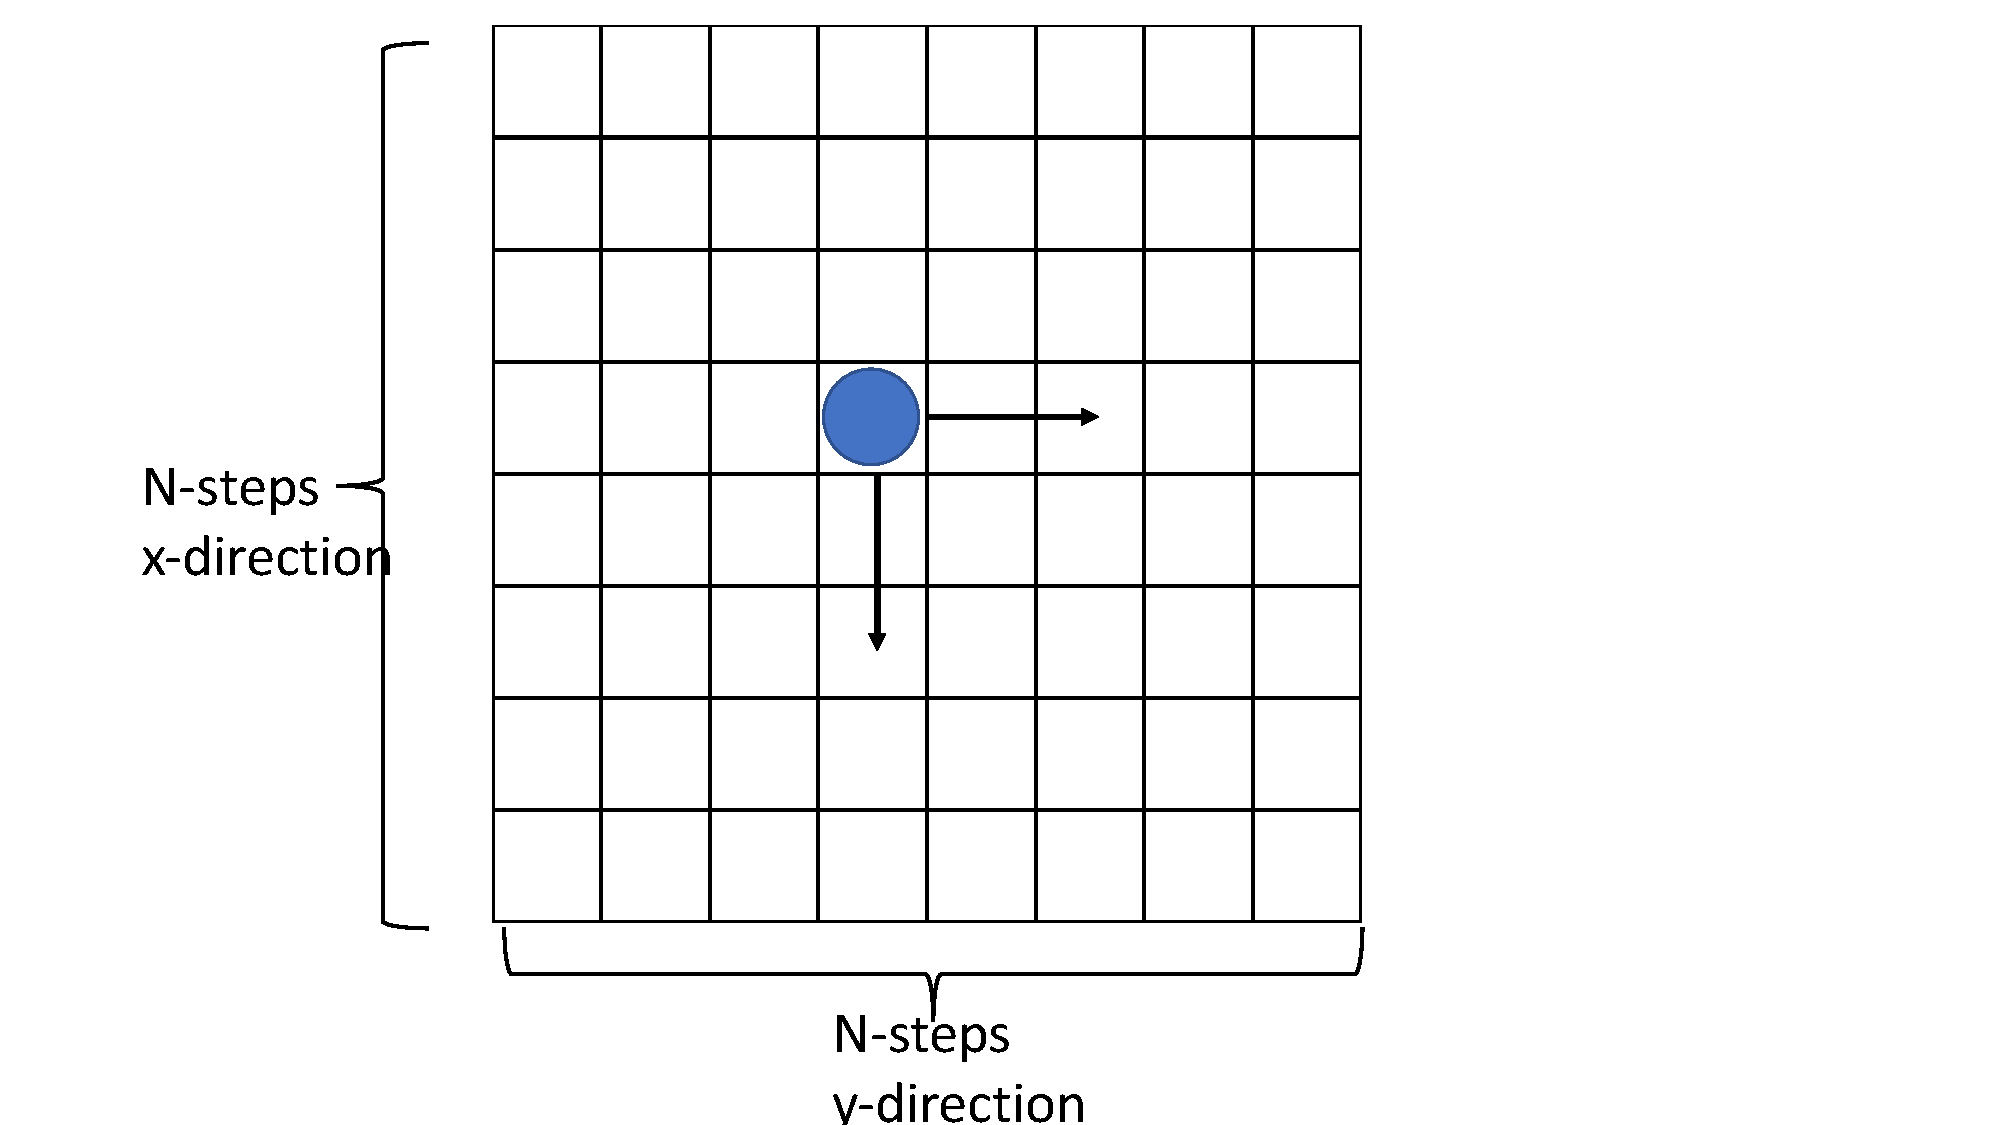
\includegraphics[width=1\textwidth]{Figures/scan.pdf}
\caption{The plane that is being scanned by the fiber tip, it is a $4x4mm$ square, that
can be scanned in N steps, where N is defined by us} 
\label{fig:scan}
\end{figure}

Another feature that is easily controlled, is the exposure time. It means we can set how many seconds, is going to be the fiber tip at
every ($i,j$) position. A greater time means more photon counted, and with a bigger amount of data of photons
counted per position, the means values per position gives a better image, with better contrast. The places where we don't have photons 
tend to have a low mean value of photons counted, while the more intense places keep counting, hence having bigger means values.
The ($i_B,j_B$) position and ($i_A,j_A$) position are related with $\vec{q}_B=(q_i,q_j)$ and $\vec{q}_A=(q_i,q_j)$ in Eq \ref{eq:quadratic} 
$\tilde{\Phi}(\vec{q}_B,\vec{q}_A)$, respectively. The spatial correlation we seek to observe. When taking a Two-photon imaging we already deduce in the 
previous Chapter that the image is going to be related with $R(\vec{r}_A)$ from Eq. \ref{eq:R}, where the ($i_A,j_A$)
 position is related with $\vec{r}_A=(x_i,y_j)$.






\subsection{Single Photon Counting Module(SPCM)}

Light is transmitted through an optic fiber from the pin hole detector to the SPCM. This 
consists in a self-contained module that detects single photons of light over the $400nm$ to $1069 nm$
wavelength range. The module used  is SPCM-AQRH-13, and it uses a unique silicon avalanche photodiode (SLiK) with a detection efficiency of more than 65\%\cite{spcm}.
The result signal coming from the SPCM are pulses where each one represents one photon.
\begin{figure}[h]
\centering
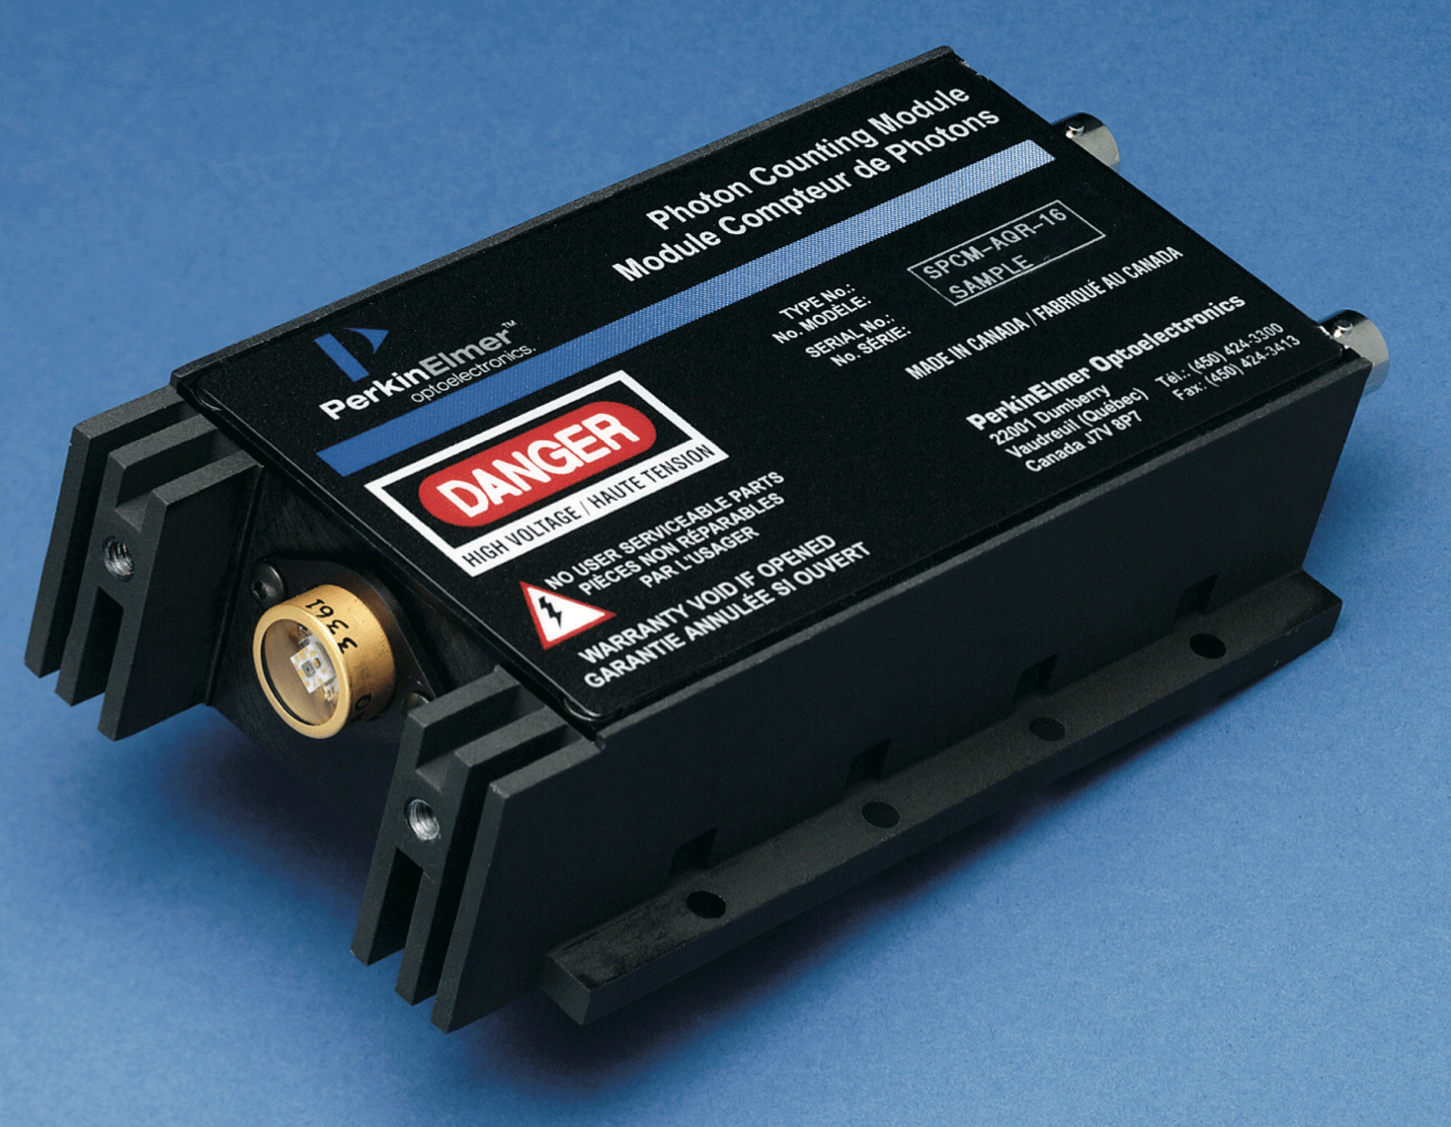
\includegraphics[width=0.35\textwidth]{Figures/spcm.png}
\caption{Single Photon Counting Module} 
\label{fig:spcm}
\end{figure}


\subsection{Field-programmable gate array(FPGA)}
Both \textit{A} and \textit{B} pulses from the respective SPCM goes to the same Field-Programmable Gate Array (FPGA). This
FPGA (ZestSC1) is programmed
to count the photon coincidences, this means that the FPGA is fast enough to detect and separate pulses from photons 
that are time-separated. 




\subsection{Computer(Data Analysis)}
LabvVIEW is used to control the detection module, and also, to recibe and translate the information
from the FPGA. It deliver the single and coincidence counts for every position in the 
scan grid, Fig. \ref{fig:scan}. Using this information is only matter of use any way to handle
this data and generate the graph for single and coincidence counts. Through this monograph
it has been used the python language and the matplotlib library to generate them.


\section{Two-Photon Imaging Setup}
Figure \ref{fig:ghostSetup} shows the extra parts of the experimental setup 
for doing Two-photon imaging. In path B we add an object and a bucket detector $D_C$. 
It may be noted that all the setups shown so far, use in essence the same optical elements.
 It is important to create an experimental setup that allows us to 
measure different things without changing it too much. For this we re-direct the light that 
goes through the object by means of a flip mirror (FM).

\begin{figure}[h!]
\centering
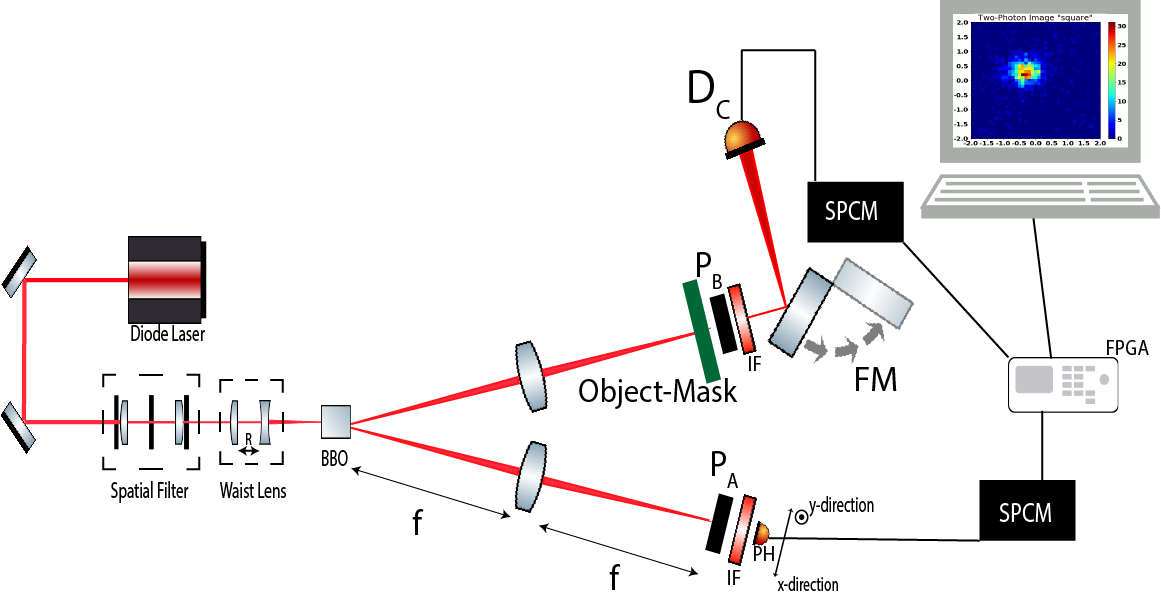
\includegraphics[width=1\textwidth]{Figures/ghostSetup2.png}
\caption{Experimental Setup for the Two-photon Imaging} 
\label{fig:ghostSetup}
\end{figure}


The object is an obstruction that is placed in the \textit{B} path. This is the object
from which we will make an image. It consist on an aperture $T(r_B)$ on a translational mount,
that allow us to move the aperture precisely in the same plane we make our detections.
This is done by manipulating a pair of screws. 
We used differents objects and in Figure \ref{fig:mask1}
there is a detailed schematic of the first one used. It consists on a square aperture placed in the 4th 
quadrant of the scanned plane. 

\begin{figure}[h!]
\centering
 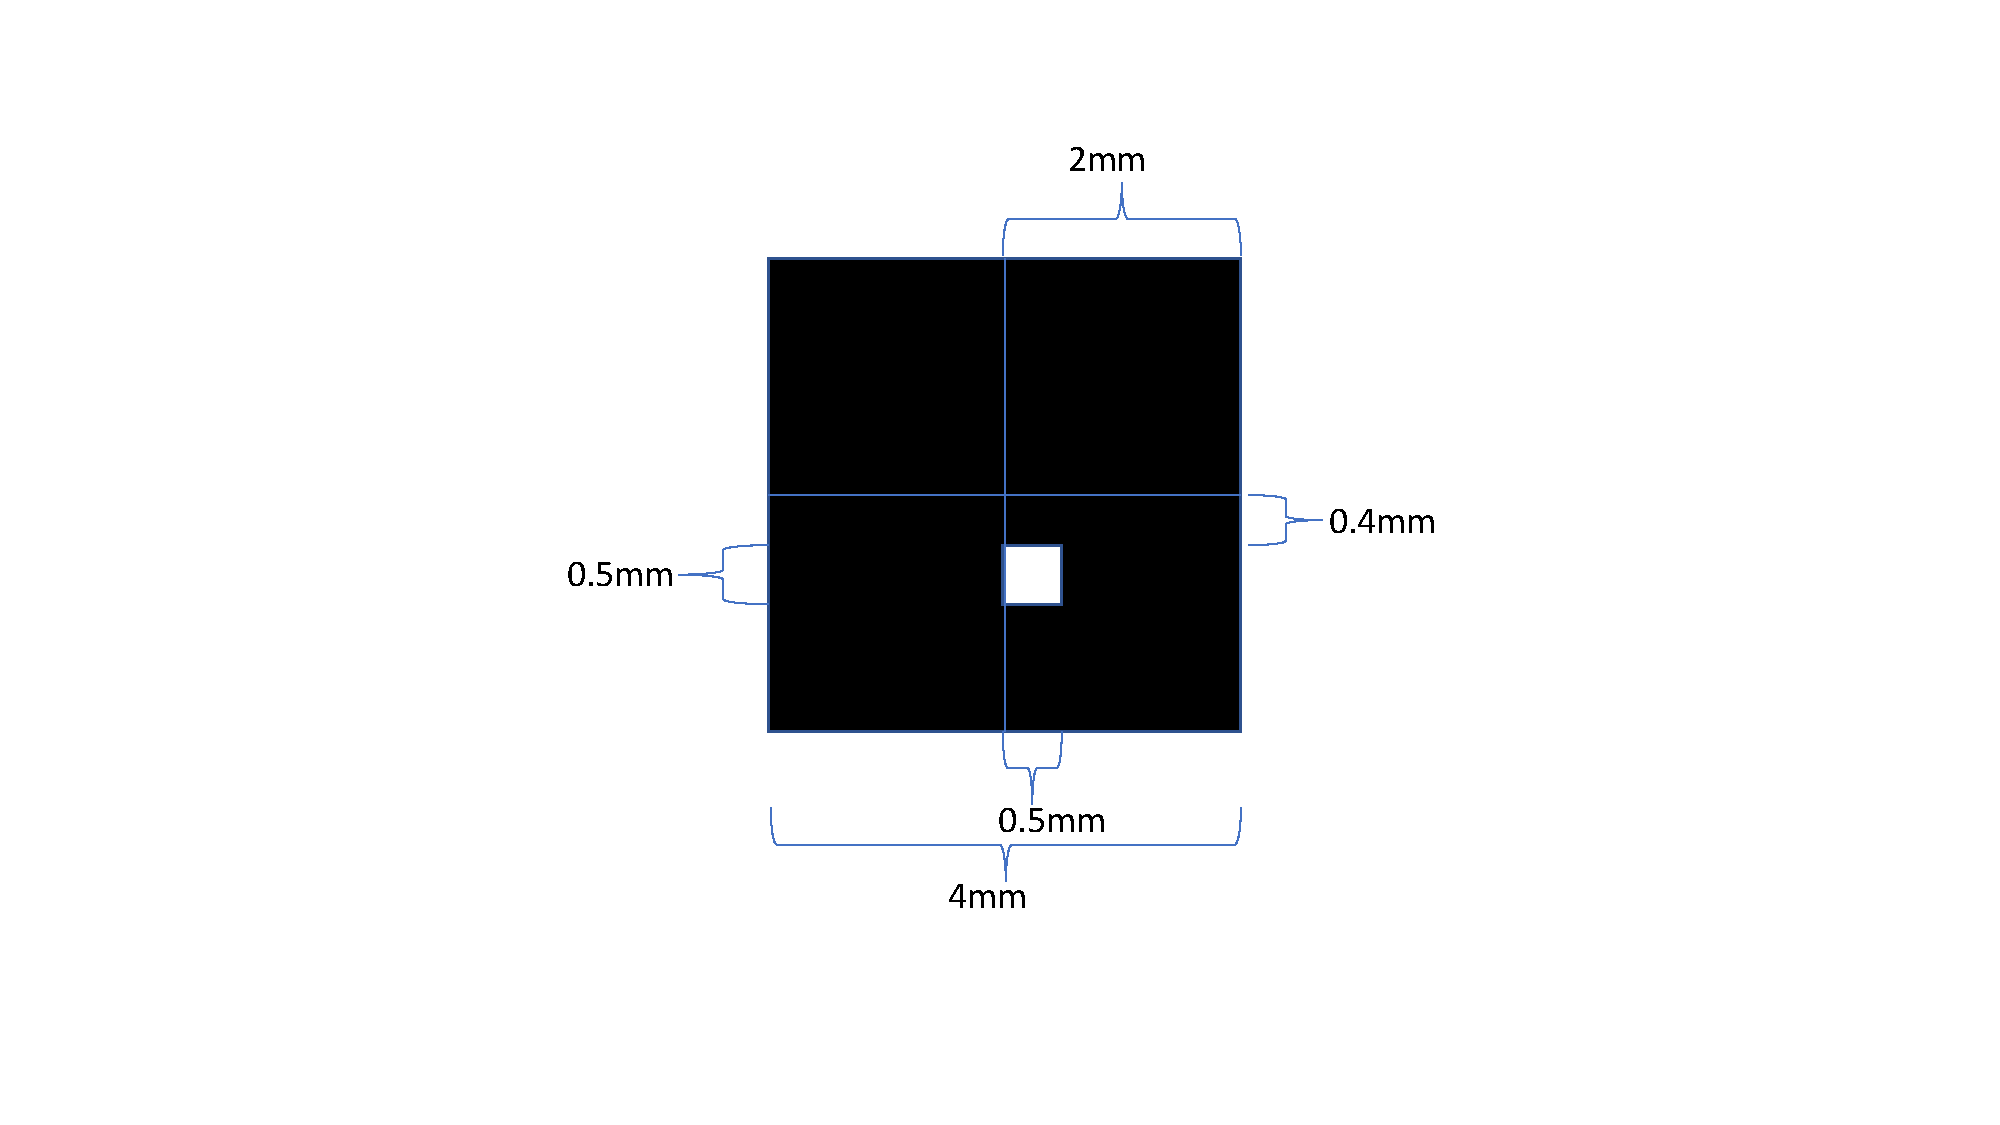
\includegraphics[width=0.6\textwidth]{Figures/mask1.pdf}
 \caption{Mask 1: Detailed description of the 'square' aperture location in the scanned plane}
\label{fig:mask1} 
\end{figure}

In Figure \ref{fig:masks} there are the other two apertures that we used so far in the 
experiment, 
these apertures were selected because of the symmetries and antisymmetries they present, 
and therefore
they helps us to recognise the effects  of the spatial correlations in the image
recovered.  

\begin{figure}[h!]
\centering
{  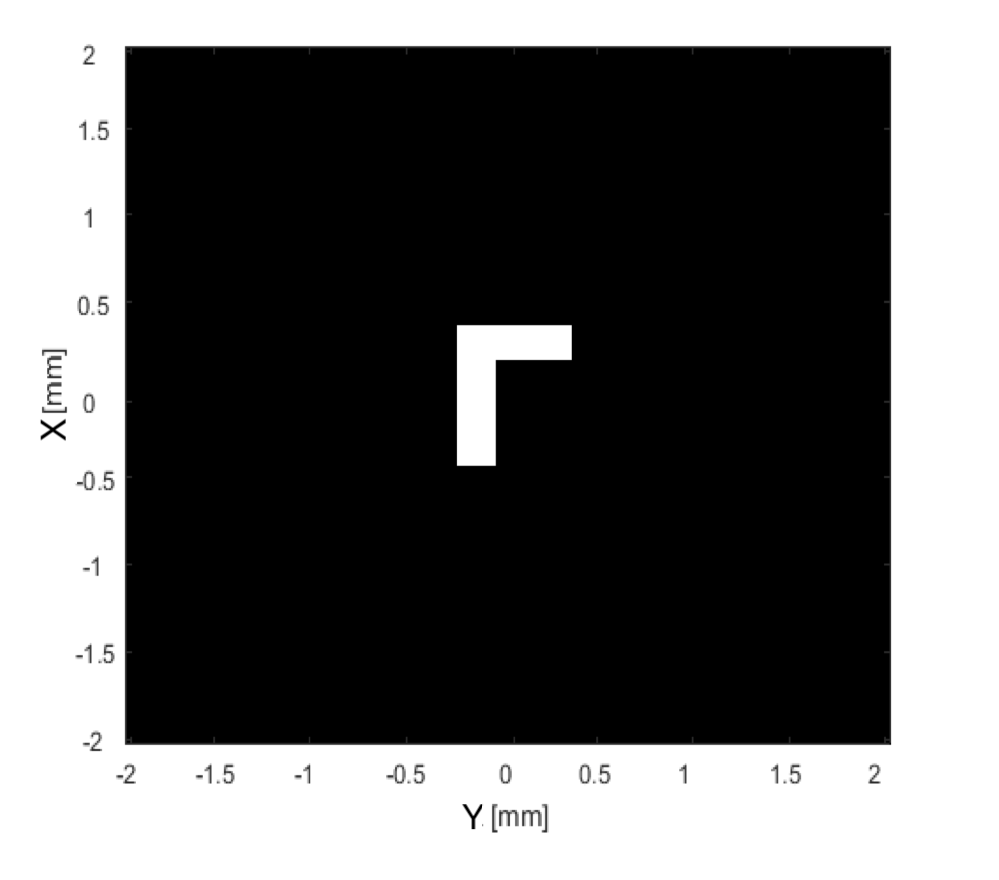
\includegraphics[width=0.45\textwidth]{Figures/mask2.png} }
{  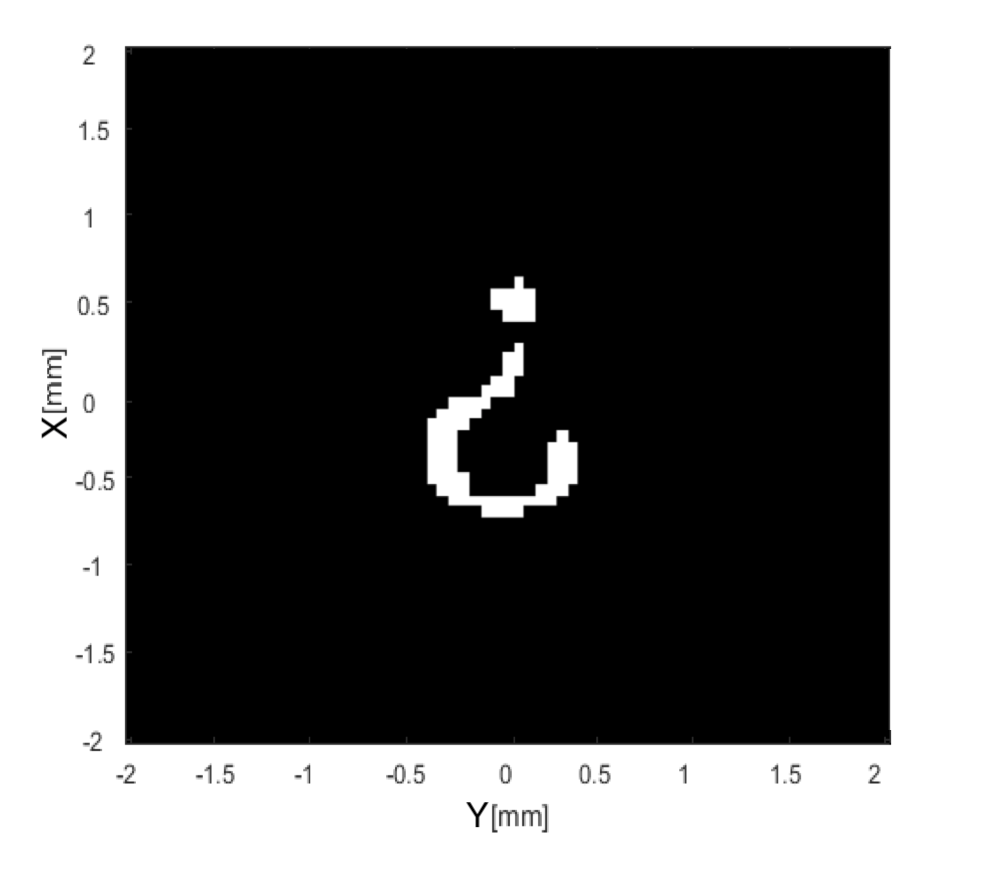
\includegraphics[width=0.45\textwidth]{Figures/mask3.png} }
\caption{Mask 2: The letter 'L' pointing down. Mask 3: Opening question mark.}
 \label{fig:masks}
\end{figure}


In order to change de path followed by the B-photon, and guide the light to a new detector $D_C$, we use a Folding mirror.
This mirror plays the role of a switch, when is up, we are know dealing with the
$D_C$ detector, and we are doing a Two-photon Imaging process. In contrast, when the mirror is 
down, we are recovering spatial information, so it is possible to recognise some sort of
shadow from the object, or to measure the spatial correlations.



The bucket detector $D_C$ consists in a coupling lens, a multimode fiber and a detector. The lens collects all the 
light that goes 
through the object couple it to the fiber that is connected to the SPCM. In contrast to the other detections made 
before with $D_A$ and $D_B$, the Bucket detector loses track of any spatial information of the photons. 